
\section{Expresiones regulares}
Una expresión regular es una expresión que describe un lenguaje de forma compacta y sencilla:

\begin{itemize}
  \item \(\varnothing\) es una expresión regular que describe el lenguaje vacío \(\emptyset\).
  \item \(\lambda\) es una expresión regular que describe el lenguaje unitario \(\{\lambda\}\).
  \item Para cada \(a\in\sigma\), \(a\) es una expresión regular que describe el lenguaje \(\{a\}\).
  \item Si \(r\) y \(s\) son dos expresiones que denotan los lenguajes \(R\) y \(S\) entonces:
        \begin{itemize}
          \item \(r|s\) ó \(r+s\) es una expresión regular que describe el lenguaje \(R\cup S\).
          \item \(rs\) es una expresión regular que describe el lenguaje \(RS\).
          \item \(r^*\) es una expresión regular que describe el lenguaje \(R^*\).
          \item \(r^+\) es una expresión regular que describe el lenguaje \(R^+\).
        \end{itemize}
\end{itemize}

\paragraph{Expresiones regulares recursivas:} Si \(r=\alpha r + \beta\), entonces \(r = \alpha^* \beta\). Además, si \(\alpha^* = \alpha^+\), entonces \(r = \alpha^*(\beta + \gamma)\) para culquier expresión regular \(\gamma\).

\subsection{Expresiones regulares a AFND-\texorpdfstring{\(\lambda\)}{Lambda}}
Dada una expresión regular \(r\), existe una AFND-\(\lambda\) \(M\) con un solo estado final y sin trancisiones a partir del mismo tal que \(\mathcal{L}(M) = \mathcal{L}(r)\).

Vamosa a demostrar por inducción sobre los operadores de las expresiones regulares.

\subsubsection{Casos base}
\begin{figure}[H]
  \begin{center}
    \caption*{\(r=\varnothing\)}
    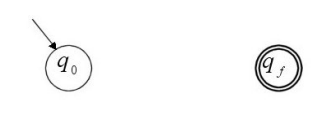
\includegraphics[scale=0.5]{imagenes/nothing}
  \end{center}
\end{figure}
\begin{figure}[H]
  \begin{center}
    \caption*{\(r=\lambda\)}
    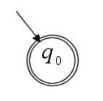
\includegraphics[scale=0.5]{imagenes/lambda}
  \end{center}
\end{figure}
\begin{figure}[H]
  \begin{center}
    \caption*{\(r=a\)}
    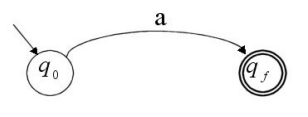
\includegraphics[scale=0.5]{imagenes/a}
  \end{center}
\end{figure}

\subsubsection{Pasos inductivos}
Sean \(r_1\) y \(r_2\) dos expresiones regulares. Supongamos que existen AFND-\(\lambda\) \\ \(M_1=\langle Q_1, \Sigma_1, \delta_1, q_1, \{f_1\}\rangle\) y \(M_2 =\langle Q_2, \Sigma_2, \delta_2, q_2, \{f_\}\rangle\) tal que \(\mathcal{L}(M_1) = \mathcal{L}(r_1)\) y \(\mathcal{L}(M_2) = \mathcal{L}(r_2)\). Vamos a armar a partir de estos autómata uno nuevo que acepte los lenguajes generados por las expresiones \(r_1|r_2\), \(r_1r_2\), \(r_1^*\) y \(r^+\).

\paragraph{\(\bm{r_1|r_2}\):} Podemos construir un automata \(M_0=\langle Q_0, \Sigma_0, \delta_0, q_0, \{f_0\}\rangle\) tal que \(\mathcal{L}(M_0) = \mathcal{L}(r_1|r_2)\) de la siguiente forma:
\begin{itemize}
  \item \(Q_0 = Q_1 \cup Q_2 \cup \{q_0, f_0\}\)
  \item \(\Sigma_0 = \Sigma_1 \cup \Sigma_2\)
  \item \(\delta_0: Q_0 \times \Sigma_0 \rightarrow \mathcal{P}(Q_0)\)
        \begin{itemize}
          \item[] \(\delta(q_0, \lambda) = \{q_1, q_2\}\)
          \item[] \(\delta(q, a) = \delta_1(q, a)\) para \(q\in Q_1-\{f_1\}\) y \(a\in \Sigma_1\cup\{\lambda\}\)
          \item[] \(\delta(q, a) = \delta_2(q, a)\) para \(q\in Q_2-\{f_2\}\) y \(a\in \Sigma_2\cup\{\lambda\}\)
          \item[] \(d(f_1,\lambda) = d(f_2,\lambda) = \{f_0\}\)
        \end{itemize}
\end{itemize}
\begin{figure}[H]
  \begin{center}
    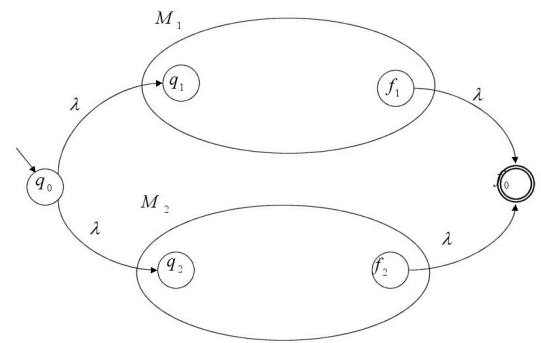
\includegraphics[scale=0.5]{imagenes/union}
  \end{center}
\end{figure}

\paragraph{\(\bm{r_1r_2}\):} \(M_0=\langle Q_0, \Sigma_0, \delta_0, q_1, \{f_2\}\rangle\):
\begin{itemize}
  \item \(Q_0 = Q_1 \cup Q_2\)
  \item \(\Sigma_0 = \Sigma_1 \cup \Sigma_2\)
  \item \(\delta_0: Q_0 \times \Sigma_0 \rightarrow \mathcal{P}(Q_0)\)
        \begin{itemize}
          \item[] \(\delta(q, a) = \delta_1(q, a)\) para \(q\in Q_1-\{f_1\}\) y \(a\in \Sigma_1\cup\{\lambda\}\)
          \item[] \(\delta(q, a) = \delta_2(q, a)\) para \(q\in Q_2-\{f_2\}\) y \(a\in \Sigma_2\cup\{\lambda\}\)
          \item[] \(d(f_1,\lambda) = \{q_2\}\)
        \end{itemize}
\end{itemize}
\begin{figure}[H]
  \begin{center}
    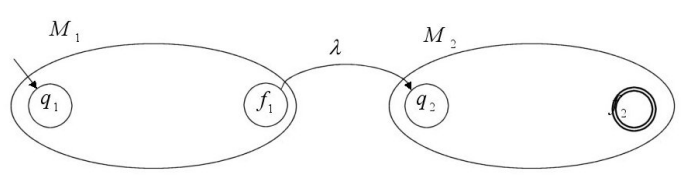
\includegraphics[scale=0.5]{imagenes/concat}
  \end{center}
\end{figure}

\paragraph{\(\bm{r_1^*}\):} \(M_0=\langle Q_0, \Sigma_1, \delta_0, q_0, \{f_0\}\rangle\):

\begin{itemize}
  \item \(Q_0 = Q_1 \cup \{f_0, q_0\}\)\
  \item \(\delta_1: Q_0 \times \Sigma_1 \rightarrow \mathcal{P}(Q_0)\)
        \begin{itemize}
          \item[] \(\delta(q_0, \lambda) = \delta(f_1,\lambda) = \{q_1, f_0\}\)
          \item[] \(\delta(q, a) = \delta_1(q, a)\) para \(q\in Q_1-\{f_1\}\) y \(a\in \Sigma_1\cup\{\lambda\}\)
        \end{itemize}
\end{itemize}
\begin{figure}[H]
  \begin{center}
    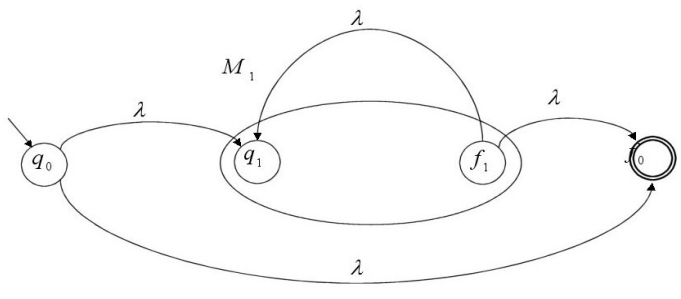
\includegraphics[scale=0.5]{imagenes/estrella}
  \end{center}
\end{figure}

Para el caso \(r_1^+\) es el mismo autómata que para este caso sin la transición \(q_0\overset{\lambda}{\rightarrow}f_0\).

\subsection{AFD a expresión regular}
\label{subsec:afd-er}
Dado un AFD \(M=\langle\{q_1, \dots, q_n\}, \Sigma, \delta, q_1, F\rangle\), que acepta el lenguaje \(\mathcal{L}\), existe una expresión regular que denota el mismo lenguaje.

\subsubsection{Demostración}
Nombremos \(R^k_{i,j}\) a la expresión regular cuyo lenguaje \(\omega \subseteq\Sigma^*\) son las cadenas que llevan al autómata \(M\) desde el estado \(q_i\) al estado \(q_j\) pasando solo por estados \(q_l\) con \(l\leq k\). En particular \(R^n_{i,j}\) es la expresión regular que representa todas las cadenas que permiten ir del estado \(i\) al estado \(j\).

Vamos a buscar como construir \(R^k_{i,j}\) para cada \(k\in\{0, \dots, n\}\) de manera inductiva. Suponiendo que demostramos la existencia de esta expresión regular, podemos concluir que la unión \(R^n_{1,f_1}|R^n_{1,f_2}|...|R^n_{1,f_m}\) (con \(f_1\dots f_m\in F\)) es la expresión regular que representa el lenguaje \(\mathcal{L}\):

\paragraph*{Caso base (\(k=0\)):} Como todos los estados están enumerados del 1 para arriba, \(k=0\) significa que no debe haber estados intermedios en el camino entre \(q_i\) y \(q_j\), por lo que pueden ser de dos formas:
\begin{itemize}
  \item Una arco del estado \(i\) al estado \(j\).
  \item Un camino de longitud cero que solo contiene el estado \(i\).
\end{itemize}

Si \(i\neq j\), entonces solo es posible la primera opción. Debemos examinar el AFD y encontrar aquellos simbolos que nos permitan ir del estado \(i\) al estado \(j\).

\begin{enumerate}
  \item Si no existe tal símbolo, entonces \(R^0_{i,j} = \varnothing\).
  \item Si existe exactamente un símbolo \(a\), entonces \(R^0_{i,j} = a\).
  \item Si existen más de un símbolo, entonces \(R^0_{i,j} = a_1|a_2|...|a_n\).
\end{enumerate}

Ahora, si \(i = j\) entonces los caminos de longitud cero también son posibles, por lo que habría que agregar a cada una de las expresiones recién mencionadas el simbolo \(\lambda\):
\begin{enumerate}
  \item \(R^0_{i,j} = \lambda\).
  \item \(R^0_{i,j} = a|\lambda\).
  \item \(R^0_{i,j} = a_1|a_2|...|a_n|\lambda\).
\end{enumerate}

\paragraph{Paso inductivo:} Supongamos que hay un camino desde el estado \(i\) al estado \(j\) que no pasa por estados mas grandes \(k\). Entonces podemos considerar las siguientes dos opciones:
\begin{enumerate}
  \item El camino no pasa por el estado \(k\), por lo que el lenguaje de \(R^{k-1}_{i,j}\) contiene a ese camino.
  \item El camino pasa por el estado \(k\) por lo menos una vez. Entonces podemos partir el camino en varias partes:
        \begin{figure}[H]
          \begin{center}
            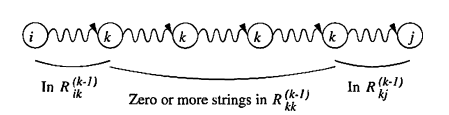
\includegraphics[scale=0.75]{imagenes/afd_regular.png}
          \end{center}
        \end{figure}
        La primer parte, va desde el estado \(i\) al estado \(k\) sin pasar por \(k\), la última parte es desde el estado \(k\) al estado \(j\) sin pasar por \(k\), y todas las partes intermedia s van desde el estado \(k\) al estado \(k\) sin pasar por \(k\). Cada una de estas partes ya tiene una expresión regular asociada: \(R^{k-1}_{i,k}\), \(R^{k-1}_{k,k}\), \(R^{k-1}_{k,j}\), por lo que podemos unirlas para obtener la expresión regular que representa el camino completo de la siguiente forma:
        \[
          R^{k-1}_{i,k}\left(R^{k-1}_{k,k}\right)^*R^{k-1}_{k,j}
        \]
\end{enumerate}

Entonces \(R^k_{i,j}\) es la unión de las expresiones de los dos tipos de caminos que acabamos de describir:
\[
  R^k_{i,j} = R^{k-1}_{i,j} \cup R^{k-1}_{i,k}\left(R^{k-1}_{k,k}\right)^*R^{k-1}_{k,j}
\]

Finalmente, si construimos en orden todas estas expresiones regulares desde \(R^0_{i,j}\), eventualmente llegaremos hasta \(R^n_{i,j}\).

Y como dijimos, más arriba si calculamos \(R^0_{1,j}\) para cada \(q_j\in F\) y unimos todas las expresiones, obtendremos la expresión regular que representa el lenguaje \(\mathcal{L}\).

\subsection{Gramática regular a AFND}
Dada una grámatica regular \(G = \langle V_N, V_T, P, S\rangle\), podemos construir un AFND \\ \(M=\langle Q,\Sigma, \delta, q_0, F\rangle\) que reconozca el lenguaje generado por \(G\)

\subsubsection{Demostración}
Vamos a constuir el autómata finito no determinista \(M\) y demostrar que reconoce el lenguaje generado por \(G\).
\paragraph{Construcción de \(M\):} Construyamos \(M\) de la siguiente manera:
\begin{itemize}
  \item \(Q = V_N\cup\{q_f\}\). Denotarmeos \(q_A\) al estado que representa al no símbolo no terminar \(A\).
  \item \(\Sigma = V_T\)
  \item \(q_0 = q_S\)
  \item Si \(A, B \in V_N\) y \(a\in\Sigma\), entonces:
        \begin{itemize}
          \item \(q_B\in\delta(q_A, a) \iff A \rightarrow aB \in P\)
          \item \(q_f \in \delta(q_A, a) \iff A \rightarrow a \in P\)
          \item \(q_A\in F \iff A \rightarrow \lambda \in P\)
          \item \(q_f\in F\)
        \end{itemize}
\end{itemize}

\paragraph{Equivalencia clausura transitiva de producciones y \(\delta\): } Vamos a probar por inducción que
\[A   \deriva \alpha B \iff q_B\in\hat\delta(q_A, \alpha)\]

\begin{itemize}
  \item \textbf{Caso base \(\alpha = \lambda\):}
        \begin{itemize}
          \item \(A\deriva \alpha B\), pero las gramáticas regulares no acentan producciones que vayan de un no terminal a otro sin pasar por un terminal, por lo que \(B = A\). Osea \(A\deriva \alpha A\).
          \item Además, como es un AFND, no tiene transiciones lambda, osea que \(\delta(q_A, \lambda) = \{q_A\}\), por lo que \(q_A\in\hat\delta(q_A, \alpha)\).
        \end{itemize}
  \item \textbf{Caso inductivo \(\alpha = \beta a\):}
        \begin{align*}
          A\deriva \alpha B   \iff            & A\deriva \beta aB \iffa{def.} \red{\exists C\in V_N: A \deriva \beta C} \wedge \blue{C\rightarrow aB} \\
          \iffab{\red{H.I}}{\blue{constr. M}} & \blue{\exists q_C\in Q, q_c\in\hat\delta(q_A,\alpha)} \land \red{q_B\in\delta(q_C,a)}                 \\
          \iff                                & q_B\in \delta(\hat\delta(q_A,\alpha),a)                                                               \\
          \iff                                & q_B\in\hat\delta(q_A, \beta a) \iff q_B\in\hat\delta(q_A, \alpha)                                     \\
        \end{align*}
\end{itemize}

\paragraph{Demostración de la equivalencia:} Vamos a demostrar que el lenguaje generado por \(G\) y \(M\) son iguales, osea que \(\alpha a\in\mathcal{L}(M)\iff S\deriva \alpha a\).
Como \(G\) es una grámatica regular, hay solo dos formas de llegar desde \(S\) hasta \(\alpha a\):
\begin{enumerate}
  \item \(\exists A\in V_N: S \deriva \alpha A \wedge A \rightarrow a \in P\)
  \item \(\exists B\in V_N: S \deriva \alpha aB \wedge B \rightarrow \lambda \in P\)
\end{enumerate}
Entonces:

\begin{align*}
  S\deriva \alpha a \iffa{def. G} & (\exists A\in V_N: S \deriva \alpha A \wedge A \rightarrow a \in P)\lor(\exists B\in V_N: S \deriva \alpha aB \wedge B \rightarrow \lambda \in P)    \\
  \iffa{Equiv. anterior}          & (\exists q_A\in Q, q_A\in\hat\delta(q_0, \alpha) \land q_f\in\delta(q_A, a)) \lor (\exists q_B\in Q, q_B\in\hat\delta(q_0, \alpha a) \land q_B\in F) \\
  \iffa{def. \(\delta\)}          & q_f\in\delta(q_S, \alpha a) \lor (\exists q_B\in Q, q_B\in\hat\delta(q_0, \alpha a) \land q_B\in F)                                                  \\
  \iff                            & \alpha a \in \mathcal{L}(M)                                                                                                                          \\
\end{align*}

Falta ver que pasa si \(\lambda\in\mathcal{L}(G)\):

\[ \lambda\in\mathcal{L}(G) \iff S\deriva \lambda \iff S\rightarrow \lambda \in P \iff q_S\in F \iff \lambda \in \mathcal{L}(M)\]
\subsection{AFD a gramática regular}
Dado un AFD \(M=\langle Q, \Sigma, \delta, q_0, F\rangle\), existe una gramática regular \(G=\langle V_N, V_T, P, S\rangle\) equivalente

\subsubsection{Demonstración}
\paragraph{Contrucción de \(G\):} Vamos a construir \(G\) de la siguiente forma:
\begin{itemize}
  \item \(V_N = Q\), para mayor claridad llamamos \(A_p\) al no terminal correspondiente al estado \(p\in Q\)
  \item \(V_T = \Sigma\)
  \item \(S = q_0\)
  \item Si \(q\in Q \land q\notin F\) entonces \(A_p \rightarrow aA_q \in P \iff \delta(p,a) = q\)
  \item Si \(q\in F\) entonces \(A_p \rightarrow a \in P \iff \delta(p,a) = q\)
  \item \(S\rightarrow \lambda \in P \iff q_0\in F\)
\end{itemize}

\paragraph{Paso intermedio:} Vamos a demostrar por inducción: \[ \hat\delta(p,\alpha) = q \iff A_p \deriva \alpha A_q\]

\begin{itemize}
  \item \textbf{Caso base:} \(\alpha = \lambda\) es trivial:
        \begin{align*}
           & \hat\delta(p,\lambda) = q \iff A_p \deriva A_p
        \end{align*}
  \item \textbf{Caso inductivo \(\alpha = \beta a\):} Queremos probar que \(\hat\delta(p,\alpha) = q \iff A_p \deriva \alpha A_q\).

        Nuestra hipotesis inductiva: \(\hat\delta(p,\beta) = q \iff A_p \deriva \beta A_q\) para todo \(|\beta| \leq n\)

        \begin{align*}
           & \hat\delta(p, \alpha) = \hat\delta(p, \beta a) = q \iffa{def.}\blue{\exists r\in Q:~\hat\delta(p,\beta) = r} \land \red{\delta(r, a) = q}          \\
           & \iffab{\blue{H.I}}{\red{constr. G}} \blue{\exists A_r, A_p \deriva \beta A_r} \land \red{A_r \rightarrow a A_q \in P} \iff A_p \deriva \beta a A_q \\
        \end{align*}
\end{itemize}

\paragraph{Demostración de equivalencia de lenguajes:}
\begin{align*}
   & \alpha a\in\mathcal{L}(M) \iffa{def.} \hat\delta(q_0, \alpha a) \in F \iffa{def.} \exists q\in Q:~\hat\delta(q_0, \alpha) = q \land \delta(q,a)\in F \\
   & \underset{\text{paso intermedio}}{\iff} \exists A_p, A_{q0} \deriva \alpha A_p \land A_p \rightarrow a \in P \iff A_{q0} \deriva \alpha a            \\
   & \underset{\text{def.}}{\iff} \alpha a \in\mathcal{L}(G)
\end{align*}
